\subsection{Design pattern utilizzati}
\subsubsection{Spring MVC}
I componenti di Spring MVC sono:
\textbf{Model:}\\
Rappresentati dalle classi che a loro volta rappresentano gli oggetti gestiti e le classi di accesso al database, nel nostro caso:
UserModel, SolutionModel, ExerciseModel, PhraseModel;
\textbf{Controller:}\\
Rappresentati da classi che rimangono “in ascolto” su un determinato URL e, grazie ai Model e alle View, si occupano di gestire la richiesta dell’utente, nel nostro caso abbiamo un solo Controller che si occuperà di demandare i rispettivi Service, che a loro volta effettueranno le operazioni sul DB attraverso i Repository.
\textbf{View:}\\ quello schifo di react!

\subsection{MongoDB Database}
\begin{figure}[H]
\centering
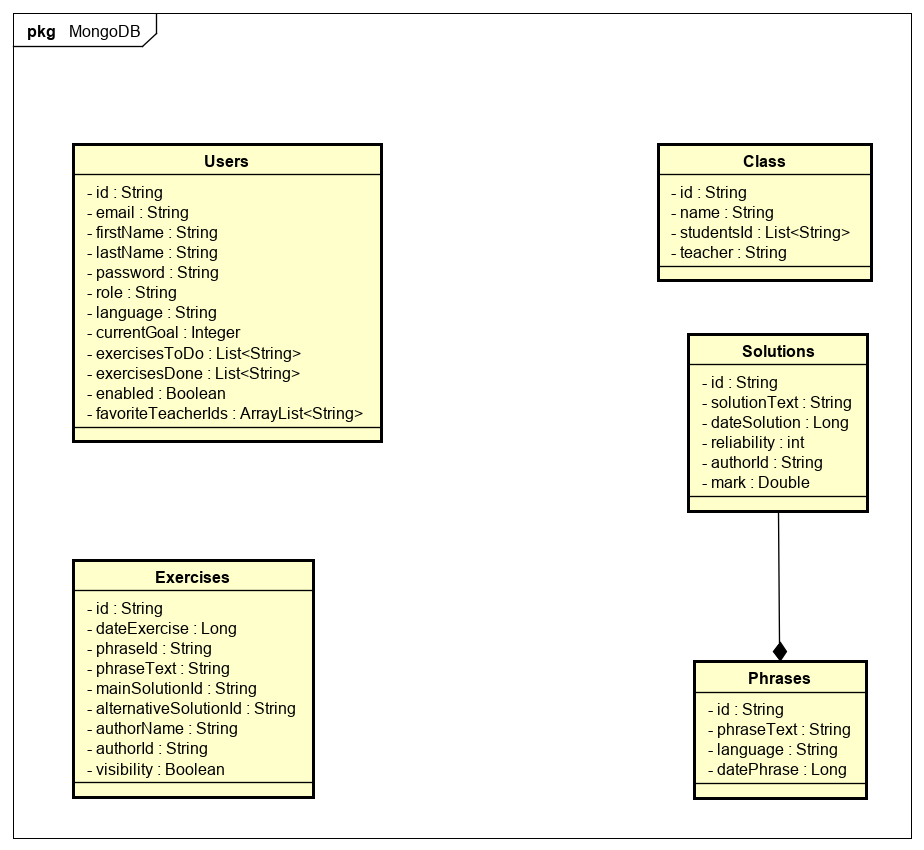
\includegraphics[width=17cm, keepaspectratio]{img/mongodb.png} 
\caption{Exercise insert}
\end{figure}